
\documentclass[microtype]{gtpart}
\usepackage{pinlabel}


%%% running feet for documentation files
\makeatletter
\def\@oddfoot{\ifnum\count0=1
\small\copyright\ Copyright 2006--11 Mathematical Sciences
  Publishers\hfill\else
\small\it Mathematical Sciences Publishers: documentation\hfill\fi}
\let\@evenfoot\@oddfoot
\makeatother

%%%% verbatim macro

\def\dq{"}   %  define a code for " so it can be used when \verb is on
\def\ttq{{\tt\dq}}  %  code for " in cmtt
%
\def\verb{\catcode`\"=\active}       %  The main
\def\brev{\catcode`\"=12}            %  switches.
%
\brev                                %  Prime switches and
\verb                                %  switch on.
%
{\obeyspaces\gdef {\ }}              
{\catcode`\`=\active\gdef`{\relax\lq}}
\def"{%
\begingroup\baselineskip=12pt\def\par{\leavevmode\endgraf}%
\tt\obeylines\obeyspaces\parskip=0pt\parindent=0pt%
\catcode`\$=12\catcode`\&=12\catcode`\^=12\catcode`\#=12%
\catcode`\_=12\catcode`\~=12%
\catcode`\{=12\catcode`\}=12\catcode`\%=12\catcode`\\=12%
\catcode`\`=\active\let"\endgroup}
%
\brev      %   Finally switch the macro off (for safety)


\def\cross{\vrule height 0.2pt depth 0.2pt width 12pt\kern -6.2pt 
\vrule height 6pt width 0.4pt depth 6pt}

%%%% metadata

\title[{\tt pinlabel}\qua A \TeX\ labelling package]{\texttt{pinlabel}\qua A \TeX\ labelling package}

\author{Colin Rourke}
\givenname{Colin}
\surname{Rourke}
\address{Mathematical Sciences Publishers\\
Department of Mathematics\\\newline
University of California\\
CA 94720-3840\\USA}
\email{contact@mathscipub.org}
\urladdr{http://www.mathscipub.org}

\volumenumber{1}
\issuenumber{}
\publicationyear{2006}
\papernumber{}
\startpage{1}
\endpage{15}

\doi{}
\MR{}
\Zbl{}

\keyword{manual}
\keyword{labelling}
\keyword{diagram}
\keyword{figure}
\subject{primary}{msc2000}{68-01}
\subject{secondary}{msc2000}{68N01}

\received{}
\revised{}
\accepted{}
\published{2006}
\publishedonline{2006}
\proposed{}
\seconded{}
\corresponding{}
\editor{}
\version{}

\arxivreference{}
\arxivpassword{}

\begin{document}

\begin{asciiabstract} 
pinlabel is a labelling package designed for attaching perfectly
formatted TeX labels to figures and diagrams in both eps and pdf
formats.  It is a tool for use by both authors and editors and can be
used both for labelling a new diagram and for relabelling an existing
diagram.  It is the recommended package for (re)labelling diagrams or
figures in papers intended for publication by Mathematical Sciences
Publishers.  The main features of the package are that it uses
coordinates read from the diagram in ghostview (or gv) and that labels
are placed with automatic and consistent spacing from the object that
they are labelling.  Many adjustment and positioning options are
provided.  The end result is a package which is easy and quick to use
and which provides accurate and eye-pleasing labelling, completely
consistent with the text.
\end{asciiabstract}

\begin{abstract} 
{\tt pinlabel} is a labelling package designed for attaching perfectly
formatted \TeX\ labels to figures and diagrams in both eps and pdf
formats.  It is a tool for use by both authors and editors and can be
used both for labelling a new diagram and for relabelling an existing
diagram.  It is the recommended package for (re)labelling diagrams or
figures in papers intended for publication by Mathematical Sciences
Publishers.  The main features of the package are that it uses
coordinates read from the diagram in {\tt GhostView} (or {\tt gv}) and
that labels are placed with automatic and consistent spacing from the
object that they are labelling.  Many adjustment and positioning
options are provided.  The end result is a package which is easy and
quick to use and which provides accurate and eye-pleasing labelling,
completely consistent with the text.

For a comparison of {\tt pinlabel} with other labelling packages which
allow one to attach \TeX\ labels, see \fullref{sec:why}.

\end{abstract}

\maketitle
\verb %%% switch on verbatim


\section{Essential ingredients}\label{sec:ess}


\subsection{Input files} 

To use "pinlabel" you need just one file "pinlabel.sty".

If you are using "latex", then you need only add the line
"\usepackage{pinlabel}" near the top of your file; if using plain
"tex" then add the line "\input pinlabel.sty" instead.  

Occasionally there will be a paragraph labelled {\small{\bf
Smallprint}}, which can safely be omitted on first reading, but which
you may need to read if problems arise.  There is a whole section of
smallprint near the end.


{\small{\bf Smallprint}\qua The package calls a standard latex package
"graphicx.sty" which all recent "tex" installations will have
available, so you should not have to worry about this.  If you are
using plain "tex" then it also calls "miniltx.tex"---a basic latex
interpreter for plain "tex"---which should also be available, but if
not, can be collected from the CTAN server.}

\subsection{Graphics files}\label{subsec:graph}

Your figures must exist either as ".eps" or as ".pdf" files.  If you
 are using only "pdflatex" then you can create and label using ".pdf"
 figures throughout if you wish.

{\small{\bf Smallprint}\qua This is a major change introduced in
 version 1.2.  In version 1.1 it was necessary to create ".eps" copies
 of all figure files.  However this {\em does not mean\/} that you can
 now safely discard the ".eps" versions for figures already labelled.
 There is a problem with bounding boxes and your labels are likely to
 move to unexpected places.  Read smallprint note \ref{subsec:bb}.}

If you are creating your figures from scratch, for example by using
 "xfig" (highly recommended) then export as ``EPS (Encapsulated
 Postscript)'' if you are using plain "tex" or if you may need to
 compile using "latex", and as ``PDF (Portable Document Format)'' if
 you are using only "pdflatex".  If you want to be able to compile
 using both "latex" and "pdflatex" then export as EPS and create a PDF
 version by running "epstopdf". The syntax is:

\medskip
"epstopdf fig.eps"

{\bf Note}\qua Do not use the similar sounding program "eps2pdf" which
may change the bounding box.

Do not draw your labels in your drawing package.


\subsection{GhostView}

You will also need a working copy of "GhostView" or "gv" or "GSview"
 for reading coordinate positions.  Most "unix" or "linux"
 installations include this program, as does "cywin" running under
 Windows, and you can collect a stand-alone copy for Windows or
 Macintosh by visiting:

\href{http://www.cs.wisc.edu/~ghost/gsview/}{\tt http://www.cs.wisc.edu/\char'176ghost/gsview/}\quad or\newline
\href{http://www.cs.wisc.edu/~ghost/macos/}{\tt http://www.cs.wisc.edu/\char'176ghost/macos/}

\section{Basic use}\label{sec:bas}

\subsection{Labelling a new figure}

Load your figure (the ".eps" version if you have made one, or the
 ".pdf" version if not) into "GhostView" or equivalent.  You will
 notice that the cursor position is recorded (in PS points) either at
 the bottom or the side.  This position is what you will read as your
 labelling coordinates.

Assuming that you are using "latex" or "pdflatex" (the changes for
 plain "tex" are indicated later) then include your figure using
 instructions as in the following typical example:

\medskip
"\begin{figure}[ht!]
\labellist
\small\hair 2pt
\pinlabel $B^3_+$ at 57 246 
\pinlabel $B^3_-$ [l] at 187 207
\pinlabel {$(S^3 \times I,A)$} [tr] at 76 26
\pinlabel $O$ [t] at 233 63
\pinlabel $K$ [r] at 125 272
\pinlabel $S^3$ [bl] at 253 283
\pinlabel $A$ [r] at 125 153
\endlabellist
\centering
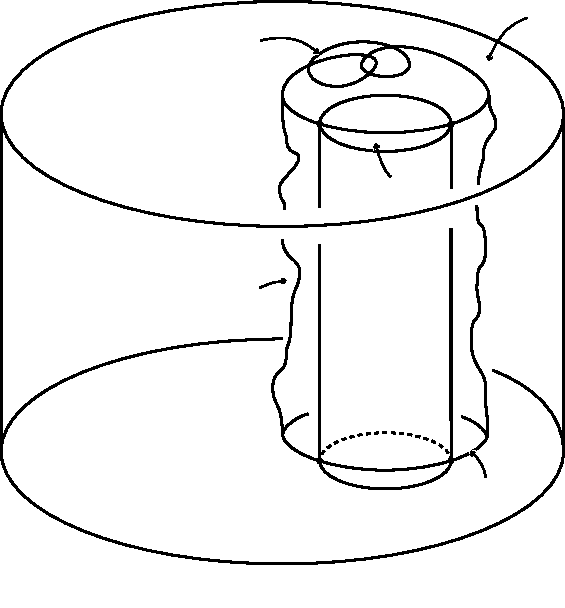
\includegraphics[scale=0.65]{fig6}
\caption{A concordance between $K$ and the unknot}
\label{fig:cobo}
\end{figure}"

The result is shown in \fullref{fig:cobo}, taken from Kim \cite[Figure
6]{kim}.

%with the unlabelled figure
%included on the left (rather smaller) for reference.  (This example is

\begin{figure}[ht!]
\centering
%\mbox{\raise 30pt\hbox{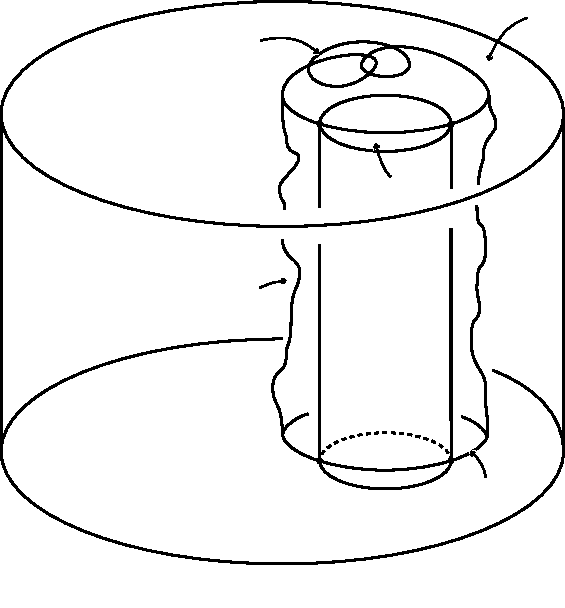
\includegraphics[scale=0.4]{fig6}}}
%\qquad\qquad
\labellist
\small\hair 2pt
\pinlabel $B^3_+$ at 57 246 
\pinlabel $B^3_-$ [l] at 187 207
\pinlabel {$(S^3 \times I,A)$} [tr] at 76 26
\pinlabel $O$ [t] at 233 63
\pinlabel $K$ [r] at 125 272
\pinlabel $S^3$ [bl] at 253 283
\pinlabel $A$ [r] at 125 153
\endlabellist
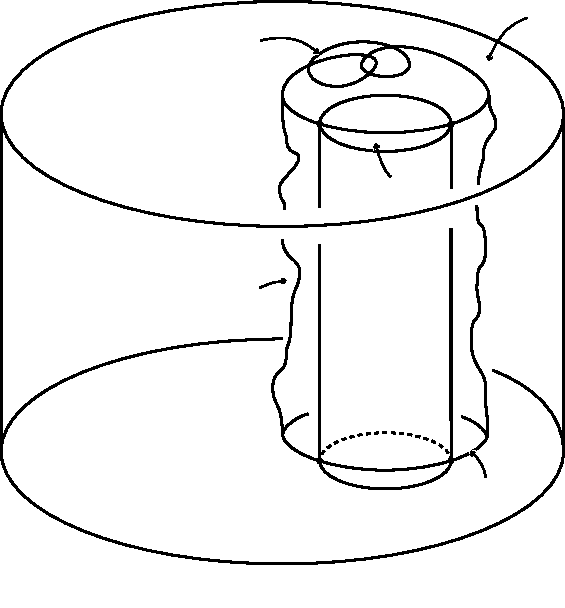
\includegraphics[scale=0.65]{fig6}
\caption{A concordance between $K$ and the unknot}
\label{fig:cobo}
\end{figure}

Let's look at this example line-by-line.  

\medskip
"\begin{figure}[ht!]" 

opens the figure environment and instructs "latex" that we want the
figure to be printed either {\bf h}ere or at the {\bf t}op of the page
({\bf !} and no-where else).  

\medskip
"\labellist"
 
opens the list of labels.  

\medskip
"\small" and "\hair 2pt" 

are formatting commands which apply to all the labels: "\small"
typesets them approximately 1 point smaller than the text
(recommended) and "\hair 2pt" adjusts the spacing between the label
and the point which is being labelled (more on this below).  Now come
the actual labels.  The first label instruction:

\medskip
"\pinlabel $B^3_+$ at 57 246" 

is the simplest form.  It tells "latex" to pin the label $B^3_+$ with
its centre at the point with coordinates $(57,246)$ in the figure.  The
remaining labels all have optional position codes.

\medskip
"\pinlabel $B^3_-$ [l] at 187 207"

tells "latex" to pin the label $B^3_-$ by the point centre-left of its
bounding box (this is what the position code "[l]" tells it to
do) at the point with with coordinates $(187,207)$.  But "pinlabel"
does not do this.  It applies automatic spacing.  The point with 
coordinates $(187,207)$ is the end of the arrow we are labelling.  We
want the label to be placed a little way away and this is what
"pinlabel" does.  It sets the label exactly 2 points away.  The "tex"
dimension "\hair" is this spacing and we just set it equal to 2
points.  The default for "\hair" is "3pt", but you can reset it to any
dimension you like for a particular label (or set of labels).  If you
want no autospacing, then use the starred form of the command:

\medskip
"\pinlabel* $B^3_-$ [l] at 187 207"

which will set the label with the centre-left of its bounding box
{\em exactly\/} at the point $(187,207)$.

The next label:

\medskip
"\pinlabel {$(S^3 \times I,A)$} [tr] at 76 26"

introduces an important point.  The label code "$(S^3 \times I,A)$"
has spaces in it.  But "pinlabel" uses spaces to separate the various
instructions, so to avoid "pinlabel" attempting to use "$(S^3" as the
label (and falling over in the process) the label must be enclosed in
braces.  The position code in this label is "[tr]" (top-right) and
this makes "pinlabel" pin this label by the point which is top-right
of the label bounding box (with autospacing) at $(76,26)$, which are
the coordinates read off from a point on the bottom curve of the
figure.  A full list of position codes will be given shortly.

In \fullref{fig:screen} is a screenshot showing how the coordinates
are read in "GSview".  The label being processed is "$S^3$", the end
of the arrow is located at $(253,283)$ and these coordinates are being
copied into the "latex" file.

\begin{figure}[ht!]
\centering
\labellist\small
\pinlabel $\cross$ <-2pt,1pt> at 428 512 
\pinlabel {{\tt GSview} cursor}  [b] <-10pt,20pt> at 428 512 
\pinlabel $\downarrow$  [b] <1pt,7pt> at 428 512 
\pinlabel $\uparrow$ [t] at 281 1
\pinlabel {coords read here} [t] <0pt,-10pt> at 281 1
\pinlabel {$\leftarrow$ coords copied here} [l] <0pt,0pt> at 753 516
\endlabellist
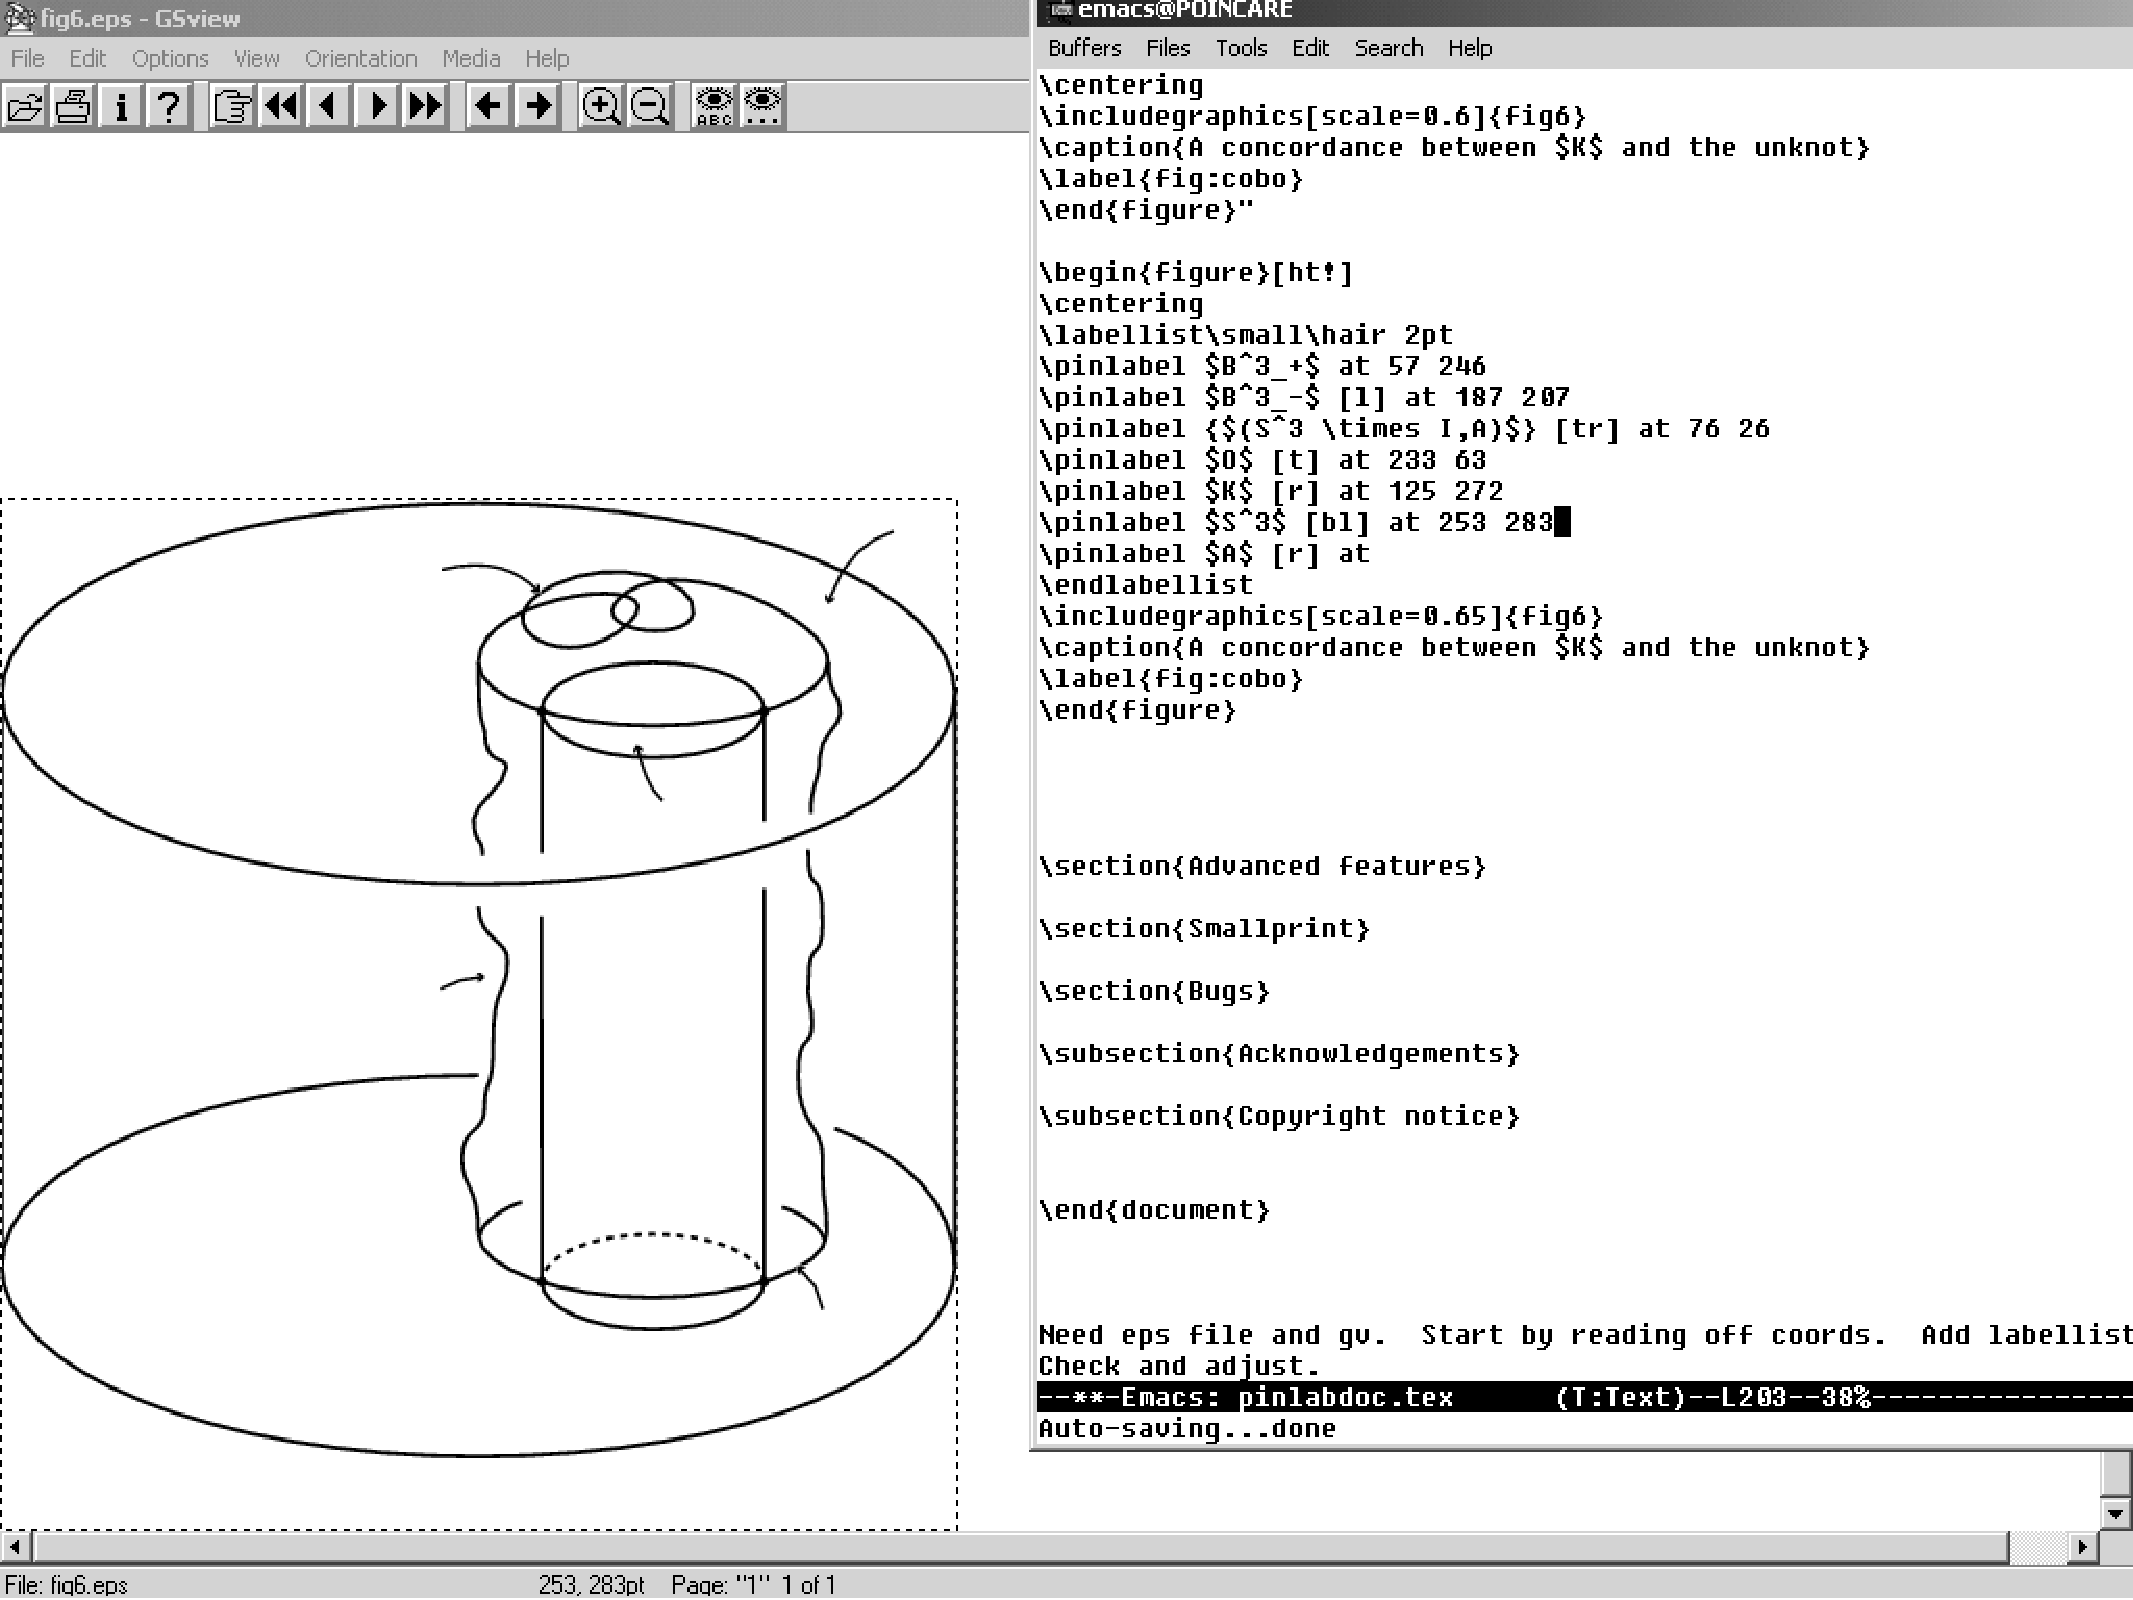
\includegraphics[width=.97\hsize]{screen}
\vspace{3mm}
\caption{Screenshot}
\label{fig:screen}
\end{figure}

In the screenshot the text editor "Emacs" is the active window on top
of "GSview" but the mouse is pointing at the point in "GSview" whose
coordinates are being read (from the bottom of the "GSview" window).
By using cursor keys in emacs, the mouse is not disturbed and the
coordinates can be copied across very rapidly and accurately.  In this
example, the transcription of the coordinates took just a couple of
minutes.

Continuing with the example, there are further labels which do not
introduce anything new and then the list of labels is closed with:

\medskip
"\endlabellist"

after which come the commands for including the figure, the caption,
the label (for cross-referencing) and for closing the "figure"
environment:

\medskip
"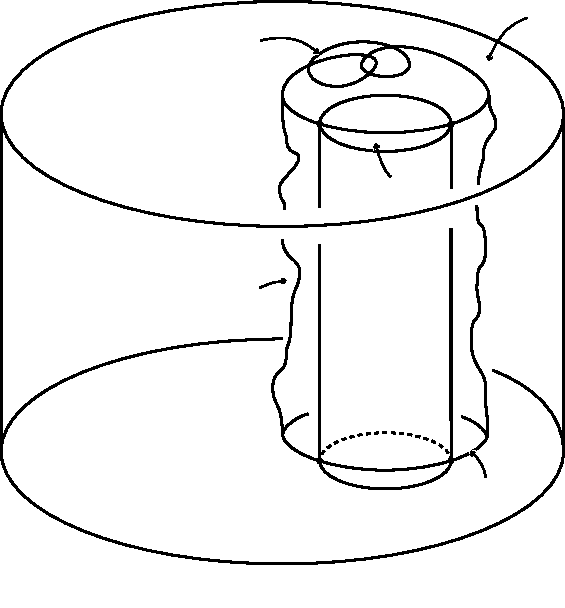
\includegraphics[scale=0.65]{fig6}
\caption{A concordance between $K$ and the unknot}
\label{fig:cobo}
\end{figure}"

\medskip {\bf Important note}\qua The filename of the figure to be
included (ie "fig6") {\em must be given without extension\/}.  The
program automatically looks for the correct file which would be
"fig6.ps" or "fig6.eps", if using "tex" or "latex", and would be
"fig6.pdf" if using "pdflatex".  If you type
"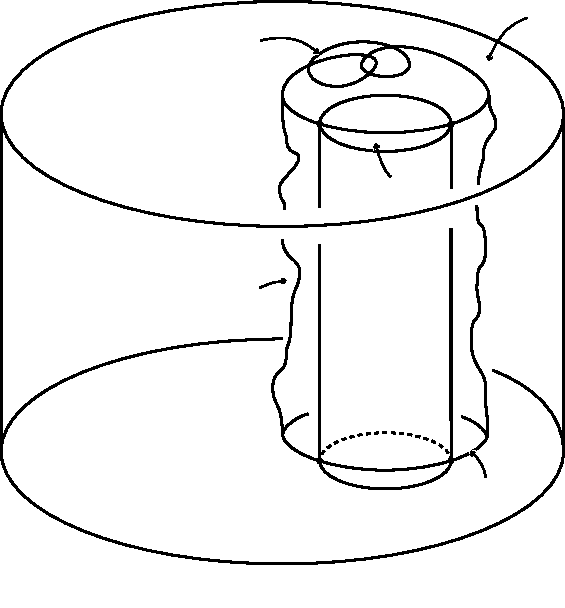
\includegraphics[scale=0.65]{fig6.eps}" then the program will give a
warning: 
 
\medskip
"cannot open figure fig6.eps.ps or .eps or .pdf on input line ..."  

and no figure will appear.



\subsection{Position codes}\label{subsec:pos}

Here is a full list of position codes: "r"=right, "l"=left, "t"=top,
"b"=bottom and "B"=baseline.  The default is centre and any sensible
combination of two codes may be give (in either order) eg
"[tl]"="[lt]"=top-left of label bounding box.  The baseline is the
line that "tex" uses for lining up characters.  In \fullref{fig:ori}
we illustrate all the possible position codes for a simple piece of
text.

\labellist\hair 1.5pt
\pinlabel "[tr]" [bl] at 162 86
\pinlabel "[br]" [tl] at 162 4
\pinlabel "[tl]" [br] at 29  86
\pinlabel "[bl]" [tr] at 29 4
\pinlabel "[t]" [b] at 96 86
\pinlabel "[b]" [t] at 96 4
\pinlabel "[r]" [l] at 162 45
\pinlabel "[l]" [r] at 29 45
\pinlabel "[Br]" [bl] at 162 21
\pinlabel "[Bl]" [br] at 29 21
\pinlabel "[B]" [b] at 96 21
\pinlabel {\Large .} at 96 21.7
\pinlabel {\Large .} at 162.3 21.7
\pinlabel {\Large .} at 28.6 21.7
\pinlabel {\Large .} at 162.3 86
\pinlabel {\Large .} at 162.3 3.7
\pinlabel {\Large .} at 28.6  86
\pinlabel {\Large .} at 28.6 3.7
\pinlabel {\Large .} at 96 86
\pinlabel {\Large .} at 96 3.7
\pinlabel {\Large .} at 162.3 45
\pinlabel {\Large .} at 28.6 45
\pinlabel {\Large .} at 96 45
\pinlabel {baseline} [l] <0pt,2pt> at 187 21
\pinlabel {$\leftarrow$ bounding box} [l] <0pt,1pt> at 162 65
\endlabellist


\begin{figure}[ht!]\small
\centering\vspace{1.5mm}
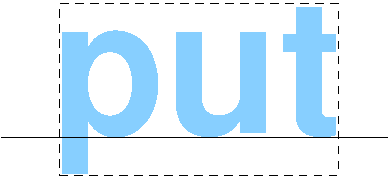
\includegraphics[width=.5\hsize]{put}
\vspace{1.5mm}
\caption{Position codes}
\label{fig:ori}
\end{figure}

If no position code is given then the label is pinned by the centre
(unlabelled dot in the figure).

\subsection{Relabelling an existing figure}

Print the figure (with its labels) as a record of how the labels go.
Then edit the ".eps" file to remove the given labels.  This is usually
easier than it sounds.  Text in a PostScript file is usually enclosed
in round brackets.  For example here is an excerpt from the file
"put.eps" used in \fullref{fig:ori}:

\medskip
"% Polyline
7.500 slw
 [60] 0 sd
n 5492 3949 m 7720 3949 l 7720 2577 l 5491 2576 l
 cp gs col0 s gr  [] 0 sd
/Helvetica-Bold ff 1500.00 scf sf
5422 3615 m
gs 1 -1 sc (put) col11 sh gr
% here ends figure;
% 
% here starts figure with depth 0
% Polyline
7.500 slw
n 5027 3649 m"

The text "(put)" is obvious and easily searchable.  In this example
``put'' is in fact a graphic element, rather than a label, so we would
not edit it out, but a label would be given in the file in a similar
format.  If ``put'' were a label to be removed, you would edit it out
by replacing "(put)" with "()".  Do the same for all labels.  Of
course if you have the source code (eg the ".fig" file for "xfig")
then you can edit the figure directly and then re-export it as an
".eps" file.

If your figure only exists as a ".pdf" file, then you can try
 coverting to ".eps" by running "epstops -eps fig.pdf" and then
 looking for text as above.  After removing labels, convert back.  If
 these dodges fail then you will have to remake the figure without
 labels using the original graphics program.

Once the old labels have been removed, relabelling is identical to
labelling a new figure as described above.




\subsection{Rotated and other exotic labels}\label{rotate}

Nothing has been said so far about the actual label.  As far as
"pinlabel" is concerned the label is just a box.  Any valid "(la)tex"
code can be used inside that box.  For example you can use a
"\rotatebox" for your label which results in a rotated label:

\medskip
"\pinlabel \rotatebox{-35}{$a^b$} at 50 30"

You could even label by another picture:

\medskip
"\pinlabel \reallyincludegraphics[height=1cm]{pic} at 50 30"

where "pic.eps" is the labelling picture.  

The reason for using the command "\reallyincludegraphics" rather than
the usual "\includegraphics" is that it has the effect of suppressing
labelling in the small picture.  This is necessary because otherwise
\TeX\ will go into an infinite loop as it tries to label by a picture,
which is in turn labelled by a picture, which \dots\ \ For more detail
about the command "\reallyincludegraphics" see the
\hyperlink{really}{smallprint note (3)} near the end of
\fullref{sec:adv}.

\fullref{fig:exotic} shows an exotic example where we have used the
whole picture as a rotated label inside itself.  The code for this
figure is as follows:

\medskip
"\begin{figure}[ht!]
\labellist\hair 1.5pt
\pinlabel \rotatebox{57}{\reallyincludegraphics[width=1cm]{put}} 
          [bl] at 162 86
\endlabellist
\centering\vspace{4.5mm}
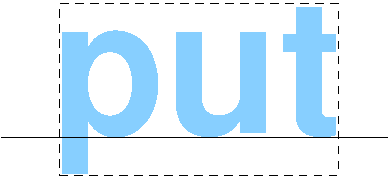
\includegraphics[width=.5\hsize]{put}
\vspace{1.5mm}
\caption{An exotic label}
\label{fig:exotic}
\end{figure}"


\begin{figure}[ht!]
\labellist\hair 1.5pt
\pinlabel \rotatebox{57}{\reallyincludegraphics[width=1cm]{put}} 
          [bl] at 162 86
\endlabellist
\centering\vspace{4.5mm}
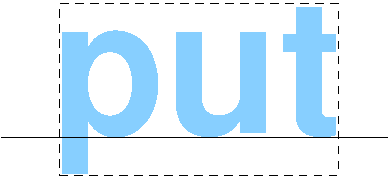
\includegraphics[width=.5\hsize]{put}
\vspace{1.5mm}
\caption{An exotic label}
\label{fig:exotic}
\end{figure}


\subsection{Using plain tex}

Since the package automatically loads "miniltx.tex", all the "latex"
commands connected with graphics will be available.  So the basic
commands for relabelling are the same.  Probably you will have a
figure inclusion macro included in whatever package you are using.
Assuming this is "\fig ... \endfig" a pinlabelled figure might look
this:

\medskip
"\fig
\labellist\ninepoint\hair 2.5pt
\pinlabel {$\partial_1 X$} [r] at 156 426
\pinlabel {$\partial_2 X$} [tl] at 334 429
\pinlabel $X_1$ at 431 513 
\pinlabel $X_2$ at 428 460 
\pinlabel $H_X$ [lb] at 311 622
\pinlabel* $H_X'$ [tr] at 178 370
\endlabellist
\centerline{\includegraphics[width=3in]{decomp}}
\centerline{Figure 23: Labelling the boundary components of $X$}
\endfig"

\section{Advanced features}\label{sec:adv}

There are three features which give the package immense flexibility in
pinning labels: pinning by coordinates, fine adjustment and the use of
an external label file.

\subsection{Pinning by coordinates}

You can pin a label by {\em any\/} point, not just by the 12 points
illustrated in \fullref{fig:ori}.  Intrinsic coordinates are defined
in the ``label-space'' by taking the origin at the centre and using
affine coordinates with horizontal unit half the width of the bounding
box and vertical half the height plus depth.  These are illustrated in
\fullref{fig:coords}.

\begin{figure}[ht!]
\centering\vspace{1.5mm}
\labellist\small\hair 1.5pt
\pinlabel $(1,1)$ [b] at 162 86
\pinlabel $(1,-1)$ [tl] at 162 4
\pinlabel $(-1,1)$ [br] at 29  86
\pinlabel $(-1,-1)$ [tr] at 29 4
\pinlabel $(0,1)$ [b] at 96 86
\pinlabel $(0,-1)$ [t] at 96 4
\pinlabel  $(1,0)$ [l] at 162 45
\pinlabel  $(-1,0)$ [r] at 29 45
\pinlabel {\Large .} at 162.3 86
\pinlabel {\Large .} at 162.3 3.7
\pinlabel {\Large .} at 28.6  86
\pinlabel {\Large .} at 28.6 3.7
\pinlabel {\Large .} at 96 86
\pinlabel {\Large .} at 96 3.7
\pinlabel {\Large .} at 162.3 45
\pinlabel {\Large .} at 28.6 45
{\hair 0pt \pinlabel {\Large .} at 96 45 }
\pinlabel $(0,0)$ [t] at 96 45
\pinlabel {\Large .} at 129 65
\pinlabel $(0.5,0.5)$ [t]  at 129 65
\pinlabel {\Large .} at 228 86
\pinlabel $(2,1)$ [b]  at 228 86
\pinlabel {\Large .} at -71 45
\pinlabel $(-2.5,0)$ [l]  at -71 45
\pinlabel {$\leftarrow$ bounding box} [l] <0pt,1pt> at 162 65
\endlabellist

\includegraphics[width=.5\hsize]{put2}
\vspace{1.5mm}
\caption{Intrinsic coordinates in label-space}
\label{fig:coords}
\end{figure}

Then the command:

\medskip
"\pinlabel* $a^b$ by -1.5 0 at 231 47"

will pin the label $a^b$ so that the point $(-1.5,0)$ in label space
(the ``label-point'') coincides with the point with (PostScript)
coordinates $(231,47)$ in the diagram (the ``diagram point'').  You
can imagine a pin inserted through the label (on an extended
transparent sheet if necessary) at the label-point and then this used
to pin the label to the diagram at the diagram-point.  This is the
reason for the name that we have adopted for the package.

We have used the starred form of "\pinlabel" in this example.  If you use
the unstarred form: 

\medskip
"\pinlabel $a^b$ by -1.5 0  at 231 47"

then the label is pinned so that the point $(-1.5,0)$ in label space
is pinned to a point exactly "\hair" away from the point $(231,47)$ in
the diagram.  The direction of this autospacing is determined by the
program.  In practice you let the program decide on this direction,
but if you want to know exactly how it decides, read part (2) of the
next smallprint.

You will now observe that there are several equivalent ways to pin
labels using standard points.  For example the following are all
exactly equivalent:

\medskip
"\pinlabel* $t-u^2$ by -1 -1  at 231 47
\pinlabel* $t-u^2$ [lb] at 231 47
\pinlabel* $t-u^2$ [bl] at 231 47
{\hair 0pt \pinlabel $t-u^2$ by -1 -1 at 231 47 }
{\hair 0pt \pinlabel $t-u^2$ [lb] at 231 47 }
{\hair 0pt \pinlabel $t-u^2$ [bl] at 231 47 }"

Note the space after the final coordinate in the above examples.  The
commands use spaces as separators and are syntax sensitive.  There
must be a space (or a line return) after the final coordinate.  The
program will attempt to recover if the syntax is wrong, but often
crashes with strange errors.  If you copy the syntax in the examples
in this file, then all will be well.  For more about syntax and errors
see \fullref{subsec:syn} and \fullref{subsec:err}.

{\small{\bf Smallprint}\qua (1)\qua The use of spaces as separators
means that the commands will not work with "\obeyspaces" set.

(2)\qua There are eight directions for autospacing: E, NE, N, NW, W,
SW, S, SE.  The choice of a discrete set of directions makes the
spacing look consistent over the diagram, whilst allowing sufficient
flexibility to space labels away from the points being labelled.  If
you use the position code "[tl]" etc then the choice of direction is
determined by the position code in the obvious way, eg "[tl]"
determines NW, ie the label is set so that the diagram-point is
"\hair" away from the label-point in the north-west direction.  The
position code "[B]" suppresses autospacing and "[Bl]" chooses W, "[Br]"
chooses E as you would expect.  When pinning by coordinates rather
than by letters, the program uses the direction (of the eight
available) closest to direction from $(0,0)$ to the label-point.  If
the label-point is $(0,0)$ then autospacing is again suppressed.  The
effect of these rules is that for example:

\medskip
"\pinlabel {label} by 1 1 at 231 56"

is not always equivalent to: 

\medskip
"\pinlabel {label} [tr] at 231 56"

If the label is rather wide, then $(1,1)$ in diagram space may be
closer to E than NE and the first command will autospace using E and
the second NE.}

\subsection{Fine adjustment}

There is an optional manual ``fine adjustment'' that can be applied to
any label which moves the label a specified amount.  This may be
inserted before "at" or directly after the label.  The adjustment
goes inside diamond brackets "<x-adj,y-adj>" where "x-adj" and "y-adj"
are arbitrary "tex" dimensions.

For example the following commands are all equivalent:

\medskip
"\pinlabel $a^b$ [l] <-2pt,1pt> at 231 47 
\pinlabel $a^b$ by -1 0  <-2pt,1pt> at 231 47 
\pinlabel $a^b$ <-2pt,1pt> [l] at 231 47 
\pinlabel $a^b$ <-2pt,1pt> by -1 0  at 231 47"

They all pin the label $a^b$ by centre-left at $(231,47)$ with two
adjustments: "\hair" (autospacing) and then "(-2pt,1pt)" manual (in other
words the label is moved 2 points to the left and 1 point upwards). 

\medskip
"\pinlabel* $a^b$ [l] <-2pt,1pt> at 231 47"

will do the same but with "\hair" set to "0pt" (ie autospacing
suppressed).  

In practice, you label your diagram as described in \fullref{sec:bas}
using either position codes or coordinates.  Then you inspect it in a
viewer and make final adjustments by (a) adjusting "\hair" (this can
be done for each label separately if necessary) and (b) adding a final
manual adjustment "<x-adj,y-adj>" again, if necessary.  For example,
inspecting \fullref{fig:cobo}, we see that the label $B^3_-$ has been
placed a little too far from the arrow tail, because of the sloping
italic type, and that $K$ is also a tad too far from its arrow because
of the shape of the letter $K$.  So to perfect the labelling you could
make fine adjustments as follows:

\medskip
"...
\pinlabel $B^3_-$ [l] <-1pt,0pt> at 187 207
\pinlabel {$(S^3 \times I,A)$} [tr] at 76 26
\pinlabel $O$ [t] at 233 63
\pinlabel $K$ [r] <1pt,0pt> at 125 272
..."

It is worth stressing that both "\hair" and the fine adjustment
"<x-adj,y-adj>" are absolute dimensions.  They do not change if the
figure is rescaled.  By contrast the coordinates of the diagram point,
"at XXX YYY", are given in PostScript points scaled by any scaling
applied to the figure and are therefore instrinsic to the figure.
This means that if the figure is rescaled, the diagram point moves
with the scaling (as you would expect) but the spacing given by
autospacing and fine adjustment stays fixed.  Thus you can make
last-minute changes of scale to a labelled diagram and the labels will
continue to be perfectly positioned.


\subsection{Using a .lab file}\label{labfile}

Labels can either be given as a list in the "tex" file (they must come
between "\labellist" and "\endlabellist") as described above or given
in the form of an external ".lab" file.  This is particularly useful
if you have a complicated diagram with labels generated by an external
program, for example the "mathfig" software, which automatically
generates ".lab" files from Mathematica input.  The syntax is identical
but the commands "\labellist" and "\endlabellist" must not be given.
The filename must be exactly the same as the figure being labelled
(but with a ".lab" extension instead of a ".eps" or ".ps" or ".pdf"
extension) and the label file must be in the same directory as the
figure file.

The program is based on "psfig" and uses "psfig" internally.  In the
examples above, we have used "graphicx" commands for figure insertion
but we could equally well have used "psfig" commands.  In the first
example, \fullref{fig:cobo} we used:

\medskip
"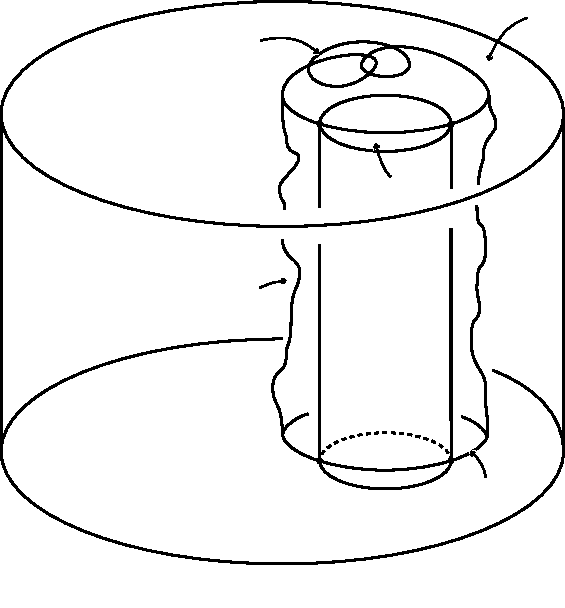
\includegraphics[scale=0.65]{fig6}"

but we could equivalently have used:

\medskip
"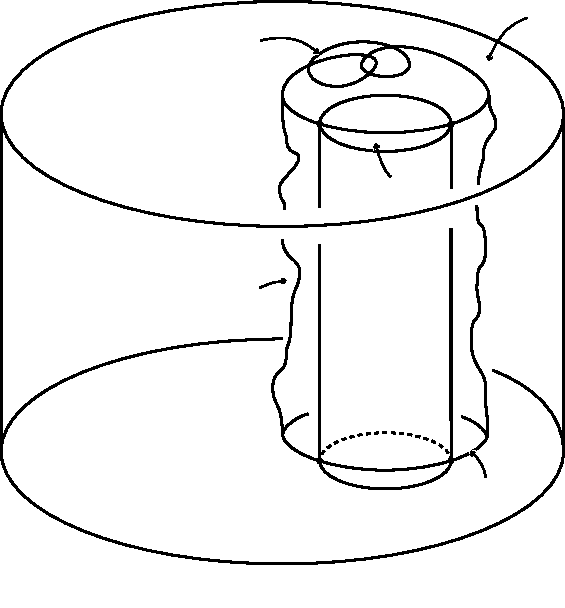
\psfig{file=fig6,scale=65}"
 
This works because the program automatically translates to "psfig"
(and adjusts the scale command correctly).  However it only does this
if there is a "labellist" waiting to be used.  This is a feature that
allows you to use "\includegraphics" in its full power (eg with
rotation) for figures that are not being pinlabelled.  But it means
that if you use an external ".lab" file then you {\em must\/} use
"psfig" syntax.  For example, suppose that your figure is "diag.eps"
in the subdirectory "figs" then if you type:

\medskip
"\centerline{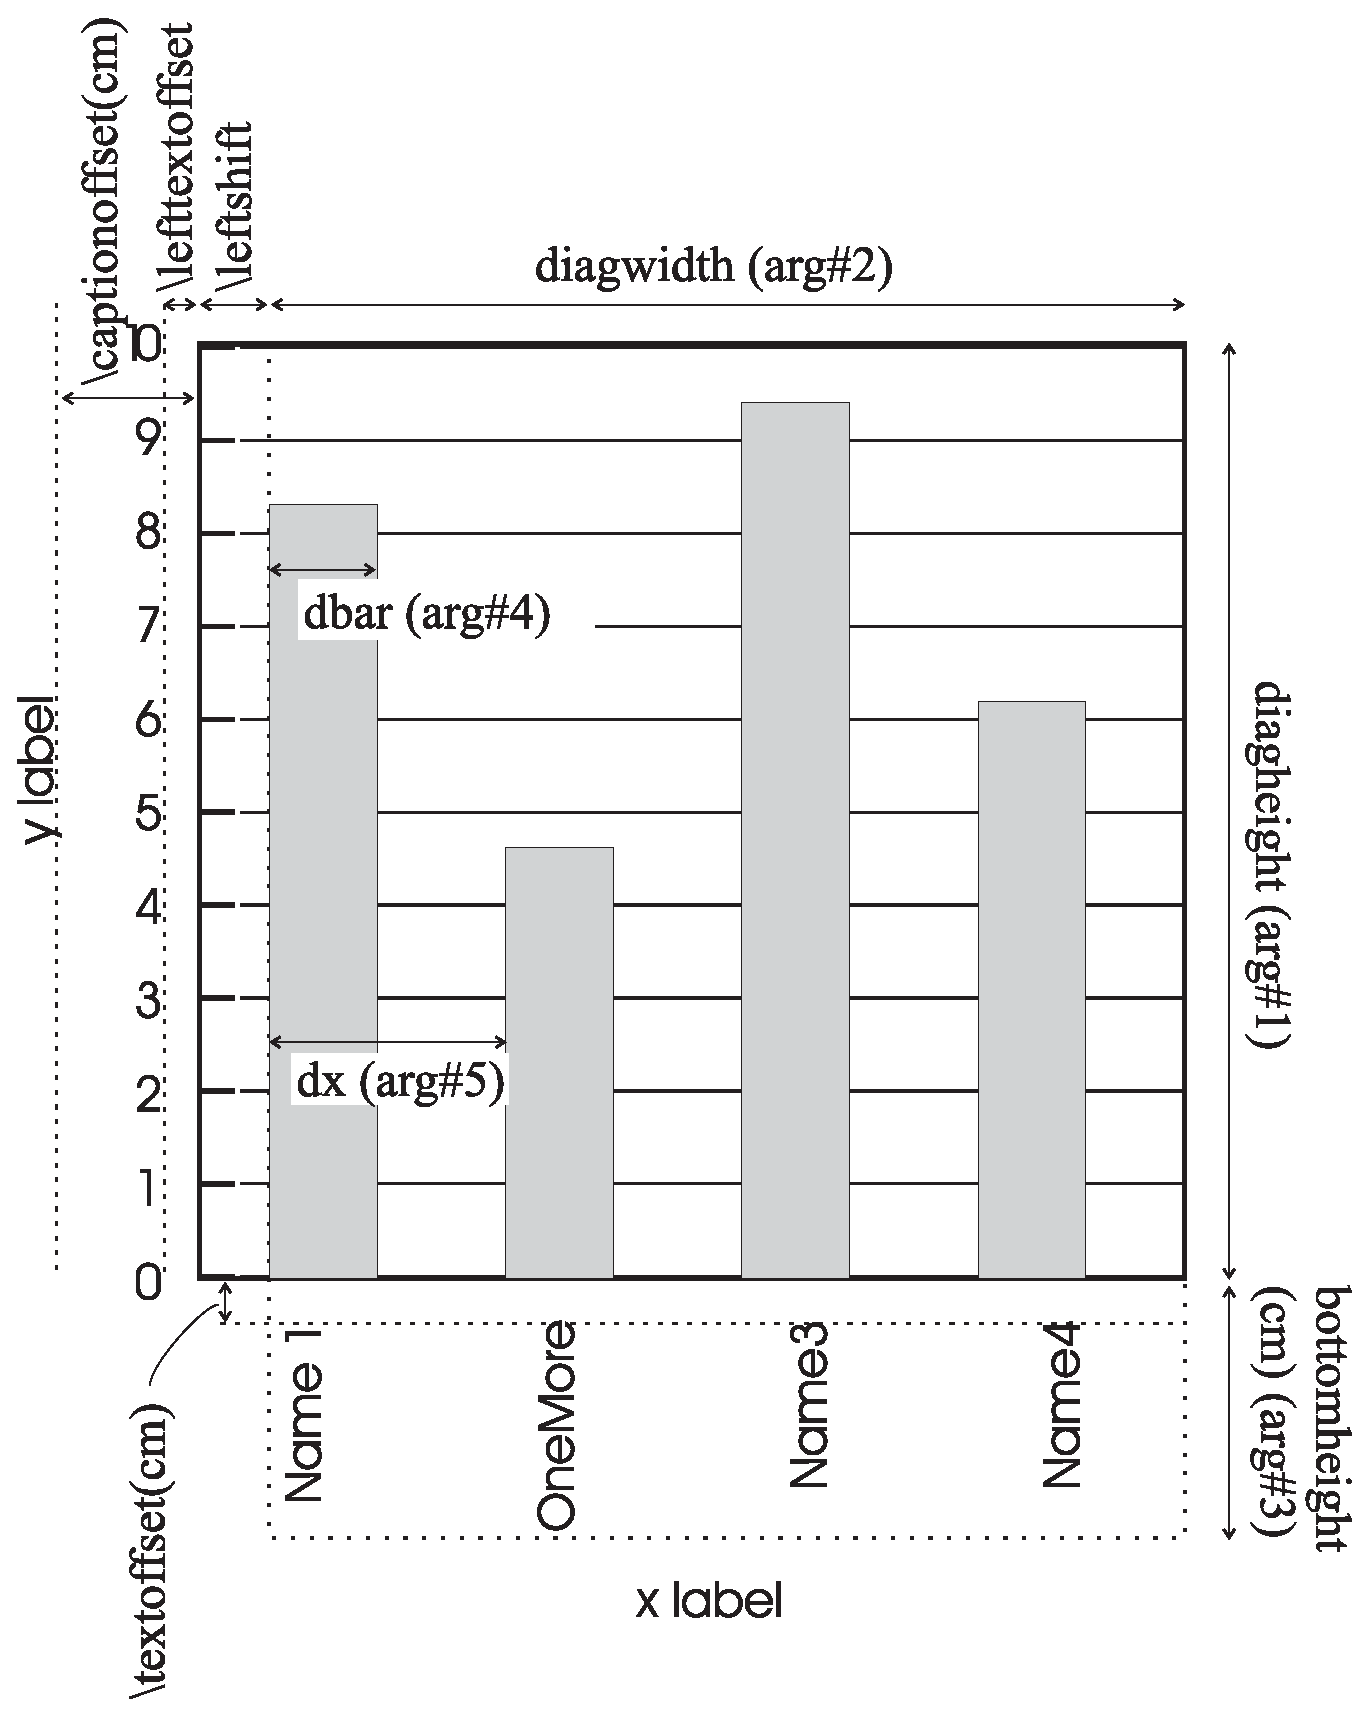
\psfig{file=figs/diag,width=.7\hsize}}"

and if the file "figs/diag.lab" reads:

\medskip
"\small\hair 2pt
\pinlabel $(-1,-1)$ [tr] at 29 4
\pinlabel $(0,1)$ [b] at 96 86
\normalsize\hair 3pt
\pinlabel $(0,-1)$ [t] at 96 4
\pinlabel  $(1,0)$ [l] at 162 45
\pinlabel  $(-1,0)$ [r] at 29 45
\pinlabel {\Large .} at 162.3 86
\pinlabel {\Large .} at 162.3 3.7"

Then these labels will be pinned to the diagram exactly as if they had
been typed in the main file.  Note the change of formatting
instructions within this list of labels.  The labels after the change
will be typeset "\normalsize" instead of "\small" with "\hair" set to
"3pt".


{\small{\bf Smallprint}\qua (1)\qua Labelling instructions do not have
to be given inside the "figure" environment.  Indeed they can be given
at any time before the next "\includegraphics" or "\psfig" command.
If there are both a "labellist" pending {\em and\/} an appropriate
".lab" file available, then the "labellist" will override the ".lab"
file (and you will get a warning to that effect).  Any formatting that
is in force when the "labellist" is typed is ignored and the
formatting that is in force inside the figure environment is used
instead.  For example the command "\small" can be given either at the
start of the "labellist" or at the start of the ".lab" file or after
"\begin{figure}[ht!]" with identical effect.  

(2)\qua Formatting instructions can be given at any stage within the
labellist or the ".lab" file as in the above example (the change of
formatting in that example would work equally well within a
"labellist").  There is a facility for setting a global format that
automatically applies to all labels.  If you type:

\medskip
"\gdef\hyperactivelabels{\small\sl\hair2.5pt}"

at the start of your file (or anywhere else you like) then all figures
that come after that line will have formatting applied exactly as if
you had typed:

\medskip
"\small\sl\hair2.5pt"
 
at the start of the "labellist" or ".lab" file.  This facility is
extremely useful for machine generated ".lab" files.  You can reset
"\hyperactivelabels" between figures.  To cancel this automatic
formatting between any two figures, type:

\medskip
"\global\let\hyperactivelabels\relax"

\hypertarget{really}{(3)}\qua You can force the program to use "graphicx" rather than
autotranslating to the appropriate "psfig" command by typing
"\reallyincludegraphics".  Since autotranslation only takes place when
there is a "labellist" pending, this will only be necessary if, for
some reason, a labellist has been supplied that applies to a later
figure.  Labelling will take not place if autotranslation is
suppressed and the "labellist" will be saved and applied to the next
figure.  An example where this was essential was given in
\fullref{rotate}.  When using a picture as a label, you need to
suppress labelling in the label or \TeX\ will go into an infinte loop


(4)\qua Autotranslation of "\includegraphics" is far from perfect.
Many of the options are not supported.  Read \fullref{sec:bugs} (on
bugs) below if you run into trouble.}
      
 
\section{Smallprint}\label{sec:smallprint}

{\small\subsection{Syntax}\label{subsec:syn}

{\bf Basic syntax}

\medskip
"\pinlabel {label} by x-pin y-pin at x-location y-location"

or

\medskip
"\pinlabel* {label} by x-pin y-pin at x-location y-location"
 
where "x-pin y-pin" is the point in intrinsic coords in label space
where we are placing the pin and "x-location y-location" is the point
in diagram space (in PS points as read in gv) where the label is
pinned.  "\pinlabel" uses "\hair" autospacing "\pinlabel*" does not. 
"\mathsurround" is set to "0pt" for parsing the label.  If the label
contains spaces, it {\em must\/} be enclosed in braces "{}".

\medskip
"x-pin", "y-pin", "x-location" and "y-location" are pure numbers, 
{\em not\/} dimensions.  The program converts them to the relevant
dimension.  The "by" and "at" are essential as are all the spaces.


{\bf Options} 

\medskip
"by x-pin y-pin" may be omitted, the default is "0 0".  

\medskip
"by x-pin y-pin" may be replaced by position codes "[r]", "[Bl]"
etc (see \fullref{subsec:pos} for full detail of these codes). 

A manual adjustment "<x-adj, y-adj>" may be added either after the label or
before "at".  Here "x-adj" and "y-adj" are "tex" dimensions, eg "5pt" or
"-2mm".  

Full examples (for more examples see earlier):

\medskip
"\pinlabel $B^3_-$ <-1pt,0pt> by -1 0 at 187 207
\pinlabel* $K$ [r] <1pt,0pt> at 125 272"


\subsection{Old syntax}\label{subsec:old}

"pinlabel.sty" is a revised version of "geompsfi.sty" and the old
syntax remains available for backwards compatibility.  The simplest
version is:  

\medskip
"\setlabel{a^b}{321}{33}{1}{1}" 

which pins the label $a^b$ by (1,1) (ie "[tr]") to $(321,33)$ with
autospacing applied.  Note that the "$$"'s for math mode are not given
with the label in this syntax.  Two new options have been added to the
old syntax.  There is a starred form:

\medskip
"\setlabel*{a^b}{321}{33}{1}{1}" 

which is the same but with autospacing suppressed, and fine
adjustments may be added:

\medskip
"\setlabel<-2pt,-1pt>{a^b}{321}{33}{1}{1}
\setlabel*<-2pt,-1pt>{a^b}{321}{33}{1}{1}"

which are the same but with a "(-2pt,-1pt)" adjustment added.

The old and new syntax may be mixed in a "labellist" or inside a
".lab" file.

{\bf Important notes}\qua (1)\qua "\mathsurround" is set to zero when
parsing the label.  This was not done in "geompsfi", so the command is
{\em not quite\/} backwards compatible.  If no "\mathsurround" is used
there is no change in label positioning.  If "\mathsurround" is used
then labels may move a small amount horizontally.

(2)\qua The label is in horizontal mode in standard ("\pinlabel")
syntax but in math mode in the old ("\setlabel") syntax, so care
should be taken if the syntaxes are mixed. 
 
\subsection{Errors}\label{subsec:err}


The program will attempt to recover from syntax errors.  Roughly
speaking, provided the "\pinlabel" command terminates with% 
" at XXX YYY" where there are spaces round the "at" and "XXX", "YYY"
are pure numbers, then the label (the code after "\pinlabel" up
to the first unbraced space) will appear in the diagram.  If the
program does not recognise the syntax between the label and the "at"
then you will get the following warning:

\medskip
"I don't understand your positioning information for label #1 and shall
ignore it; or perhaps your label has a space and needs braces."

where "#1" is replaced by the actual label code.  If there is no "at"
then the program has a harder time recovering but you should get the
following warning:

\medskip
"There is something wrong with your syntax for label #1;
you must finish with "\ttq" at XXX YYY"\ttq" : the "\ttq"at"\ttq" and spaces are important!
I'm going to try to ignore this label: don't blame me if there are some
funny numbers in your diagram and later labels are out-of-position."

By looking at the finished diagram, you should be able to pick out
where the error lies.  If all that is wrong with the syntax is that
the position code has been mistyped then you should just get the
following warning:

\medskip
"Unknown position code [#2]; I shall ignore it."

where "[#2]" is the mistyped code.  If you make a basic "tex" error
(unmatched "$..$"'s for example) then you should get an error 
"missing $" or similar.   If all else fails, check each "\pinlabel" 
command against the samples given here.

\subsection{Bounding boxes}\label{subsec:bb}

In \ref{subsec:graph} it was mentioned that conversion from ".eps" to
 ".pdf" may change the bounding box.  In a ".pdf" file the bounding
 box always has bottom-left corner at "0 0" but this is not true for
 an ".eps" file.  The recommended converter "epstopdf" does not change
 the {\em size} of the bounding box but merely moves the bottom-left
 corner to "0 0".  This implies that an ".eps" file used to position
 labels can safely be discarded if and only if the bottom-left corner
 in the bounding box in the ".eps" file is in fact at "0 0".

 
If you need to know the deep detail on how "pinlabel" reads the
 bounding box, read on.  If a bounding box is supplied via options to
 "\includegraphics" or "\psfig",  eg

{\footnotesize\medskip
 "\includegraphics[bbllx=10bp,bblly=12bp,bburx=150bp,bbury=273bp,width=2in]{fig}",}

 which specifies the box "10 12 150 273" (the "bp" specifies
 postscript points), then this specification is used {\em whatever the
 actual bounding box is for the graphics files.}  Otherwise pinlabel
 looks for a file named "fig.ps" or "fig.eps" or "fig.pdf" {\em in
 that order}.  If it finds such a file, it reads the bounding box and
 uses that.  If there is no file "fig.ps" or "fig.eps" or "fig.pdf" or
 if "pinlabel" cannot find a bounding box in the first of these that
 exists, then you get an error message and no figure is typeset.}




\section{Bugs}\label{sec:bugs}

No spaces are permitted in the file argument of "\psfig".
Autotranslation of "graphicx" means that no spaces are permitted in
the file argument to "\includegraphics". \newline Thus
"\includegraphics[width=4in]{ foo }" will produce errors.  It should
be typed "\includegraphics[width=4in]{foo}".  Spaces are permitted
with other arguments.
          
Many of the options in "graphicx" are not supported by
 autotranslation.  The supported ones are: "width", "height", "scale",
 "bbllx", "bblly", "bburx", "bbury" and "clip".  The syntax for clip
 is "clip=".  Replace "keepaspectratio=true" by "proportional=".  The
 arguments to "bbllx" etc must be specified in postscript points (see
 the example above).

\medskip
"\graphicspath{}" is not supported.               

Automatic configuration for "dvips" and "pdflatex" is included in the
program.  No support is provided for other drivers.
 
The program is fully compatible with plain "tex" via the "latex"
interpreter "miniltx.tex" written by David Carlisle.  It works with
"dvips" but {\em not\/} with "pdftex".  For pdf output from plain
"tex" use "dvips" followed by "ps2pdf".

{\bf Note}\qua "\psfig" ouputs a vbox, which is not centred in the
"latex" "{center}" environment.  Either use "\centerline{}" or type
"\leavevmode" before "\psfig{..}".  The translator adds "\leavevmode"
for "\includegraphics", which therefore centres correctly as usual
in the "{center}" environment.

\section{Why pinlabel?}\label{sec:why}

This section reviews other labelling packages and attempts to answer
the obvious question: why do we need a new package?  Well the first
obvious comment is that the package is not new.  It is the old package
"geompfsi", rewritten, with extra functionality and new syntax.
However it is fully backwardly compatible and all "geompfsi" diagrams
should compile perfectly with "pinlabel" (with one small caveat, see
note (1) in \fullref{subsec:old}).


\subsection{rlepsf and psfrag}

Turning to other packages which are capable of perfect \TeX\ formatted
labels, there are two relabelling packages "rlepsf" and "psfrag" which
replace dummy labels in the ".eps" file with "tex" labels specified in
the ".tex" file.  Both of these are incompatible with "pdflatex",
which makes them now unsuitable for figures created from scratch.
They depend on low level interfacing with PostScript via "\special"
commands.  Indeed both are somewhat sensitive as to the precise nature
of the ".eps" file being relabelled.  If you have a file with figures
relabelled using "rlepsf" or "psfrag", the most robust way to make it
"pdflatex" compatible is to relabel the figures using "pinlabel".
(But you can also treat the figures like "pstricks" figures etc, see
\fullref{subsec:pst}.)


\subsection{Combined output from xfig}

\medskip
"xfig" is capable of creating figures with properly formatted "tex"
 labels using "combined ps/latex (pstex)" or "combined pdf/latex"
 output.  This works well, and existing figures using this system can
 be used with "pdflatex" with only minor changes: if you export as
 "combined ps/latex (pstex)" you have to rename the ".pstex" file
 (which is in fact an ".eps" file) to an ".eps" file and convert to
 ".pdf" and in both cases you have edit the "\includegraphics{}"
 command to remove the ".pstex" or ".pdf" extension.

However starting from scratch, it is much more efficient to create
 unlabelled ".eps" or ".pdf" files in "xfig" and then add labels with
 "pinlabel".  The positioning of the labels in "xfig" is hit-and-miss
 and difficult to adjust: you have to keep the ".fig" file open, move
 the label a little, re-export, reconvert to ".pdf", recompile, repeat
 \ldots. Using "pinlabel" the label is usually positioned perfectly
 first time and can be adjusted without reopening "xfig", which is far
 more efficient.


\subsection{overpic, labelfig, xyoverpic and WARMreader}

There are three packages which, like "pinlabel" add the labels as an
overlay on an existing ".eps" figure and therefore produce robust code
suitable for "pdflatex".  "overpic" is the most basic.  Reading label
positioning is pure guesswork (using a simple grid) and there are no
fine adjustments for positioning, which makes the final tuning very
time-consuming (and highly sensitive to any last-minute change of
scale).  "labelfig" is slightly more sophisticated, but reading label
positioning is the same guesswork as for "overpic", there are some
position codes, but again there is no fine adjustment and moreover
the syntax is {\em awful\/}:

\medskip
"\SetLabels
\E(.18*.68) $F$\\
\E(.39*.68) $G$\\
...
\E(.75*.2) or\\
\E(.88*.2) $F$\\
\endSetLabels
%\ShowGrid
\AffixLabels{\BoxedEPSF{Mutant.ART scaled  500}}}"

\medskip "xyoverpic" is much more sophisticated, offering a good deal
of the functionality of "pinlabel".  But accurate positioning of
labels requires a preprocessor such as "WARMreader".  You can also
read the label positions using "ghostview" but you have to be clever
to do this.  Firstly you need to make sure that your ".eps" file has
its bounding box starting at "(0,0)" then you need to supply the other
bounding box coordinates directly after "\begin{xyoverpic*}" (they are
"(280,210)" in the example below) to set the scaling; then the
"ghostview" coordinates can be used.  The syntax for the actual labels
is, if anything, worse than "labelfig" but it does have both a
position code and an element of fine positioning built in:

\medskip
"\begin{xyoverpic*}{(280,210)}{scale=0.75}{figures/pgl-orbifold}
 ,(0, 107)*++!R{4}
 ,(64,178)*++!DR{4}
 ,(278,107)*++!L{2}
 ,(130, 136)*++!LD{2}
 ,(172,107)*++!U{3}
\end{xyoverpic*}}"

By contrast, "pinlabel" uses "ghostview" coordinates for files whose
bounding box does not start at "(0,0)" and the syntax is transparent.

\subsection{Summary}

To summarise the advantages of "pinlabel" over existing packages which
do a broadly similar job: only "xyoverpic" with the the tweaks
described above (or with "WARMreader" input) gets location in diagram
accurate first time.  But it is marred by impossible syntax and
limited fine adjustment.

\medskip "pinlabel" gets a similar accuracy in positioning and has
transparent syntax and arbitrary fine adjustment.  Moreover "pinlabel"
has a powerful feature not shared by any other package: the ability to
pin labels using arbitrary pin positions, specified in instrinsic
coordinates in the label.  This has not been stressed in this manual
because it is rarely necessary in hand constructed diagrams, but for
machine generated code it is very useful indeed.  For example Silvio
Levy (who originated this feature) writes:

{\leftskip 15pt\rightskip 15pt\leavevmode\llap{``}{\em I find it very convenient to
place (small, "mathematica"-generated) labels around a circle, say, by
pinning the label at $(-\cos\theta,-\sin \theta)$ in label
coordinates.  This works very well.}''\par}

\subsection{pstricks, eepic, specials}\label{subsec:pst}

Before leaving the topic of other packages, there are a number of
packages which, like "rlepsf" and "psfrag" interface directly with
PostScript.  All are unsuitable for use with "pdflatex" for this
reason.  If faced with a file containing such figures, you need to
precompile the figures using "latex" then "dvips -E" (or "dvips"
followed by "ps2epsi", which is more robust about bounding box
placement) and then "epstopdf" to produce a ".pdf" file for inclusion
in the usual way.


\section{Pinlabeler and labelpin}

Peter Storm has written an extremely useful extension to "gv", called
 "pinlabeler" which automatically copies the coordinates of the cursor
 in "gv" to a text file open for editing.  To be precise it writes a
 line like:

\medskip
"\pinlabel {$$} [] at XXX YYY "

into the file at the position of the cursor (in the editor) where 
 " XXX YYY " are the PS coordinates of the cursor in "gv".  It does this
 when you click on a point in the "gv" window.  This makes
 transcribing coordinates much simpler: you just click on the label
 position and then fill in the label and positioning code.

You can find full details (including installation instructions) at:

\href{http://hans.math.upenn.edu/~pstorm/pinlabeler.html}{\tt
 http://hans.math.upenn.edu/\char'176pstorm/pinlabeler.html}


Nathan Dunfield has written a similar program "labelpin", which is a
 python script and therefore, unlike Storm's program, does not need
 compilation.  Both work perfectly with "cygwin" under Windows
 ("pinlabeler" comes ready compiled for "cygwin") and both work
 perfectly with ".pdf" figures, moreover "labelpin" works on a Mac.

The script and instructions for "labelpin" can be downloaded from:

\href{http://www.math.uiuc.edu/~nmd/software/}{\tt
 http://www.math.uiuc.edu/\char'176nmd/software/}




\section{Acknowledgements and copyright notice}

"pinlabel" is based on "geompsfi.sty" written by Silvio Levy which in
turn is based on "psfig.sty" written by Trevor Darrell.  Their
agreement to this development is gratefully acknowledged.  Silvio Levy
has made several helpful suggestions and done extensive testing and
debugging.  

Thanks also to Walter Neumann, Paulo Ney de Souza, Nicholas Jackson
 and Noam Shomron for helpful suggestions, testing and debugging, and
 also to Mark Peletier for providing the code that reads the bounding
 box from a ".pdf" file, thus making ".eps" versions of figure files
 unnecessary when using "pdflatex".

\subsection*{Copyright notice}


The following notice appears at the start of the source file:

{\small
\medskip
"
     Copyright 2006-11 Mathematical Sciences Publishers (MSP)

                              NOTICE
  
  This package may be distributed and/or modified under the 
  conditions of the LaTeX Project Public License, either version 
  1.3 of this license or (at your option) any later version.
  The latest version of this license is in"

\noindent\hspace{1in}\href{http://www.latex-project.org/lppl.txt}{{\tt http://www.latex-project.org/lppl.txt}}

\medskip
"  and version 1.3 or later is part of all distributions of LaTeX
  version 2005/12/01 or later.

  This package has the LPPL maintenance status `maintained' and is
  currently maintained by MSP: contact@mathscipub.org 

  It comprises the files: pinlabel.sty (this file) and the manual
  pinlabdoc.pdf where full documentation may be found, together with
  the source files for the documentation."}



\begin{thebibliography}

\bibitem{kim}
\textbf{H\,J Kim}, \href{http://dx.doi.org/10.2140/gt.2006.10.27}{\emph{Modifying surfaces in 4--manifolds by twist spinning}}, Geom.
  Topol. 10 (2006) 27--56

\end{thebibliography}

\end{document}

